\documentclass{article}
\usepackage{polski}
\usepackage[utf8]{inputenc}
\usepackage{graphicx}
\usepackage{listings}
\usepackage{hyperref}
\usepackage{graphicx}
\graphicspath{ {../images/} }
\setlength\parindent{0pt}

\title{%
  Techniki kompilacji - dokumentacja końcowa \\
  \large Prowadzący - dr inż. Piotr Gawkowski
}
\author{Tomasz Nowak}
\date{}

\begin{document}

\maketitle


\section{Opis języka}

\subsection{Wstęp}
"LOGO z L-systemem" - interpreter języka \textit{LTurtle} pozwalającego definiować L-system i opisywać elementarne operacje w tym systemie w języku “grafiki żółwia”.
\newline{}
Podstawowe elementy języka:
\begin{itemize}
    \item{Funkcje wbudowane, zmieniające stan rysującego żółwia}
    \item{Zbiór symboli, każdy z nich reprezentuje pewien ciąg operacji żółwia}
    \item{Zbiór produkcji, generujących ciągi symboli w L-systemie}
\end{itemize}
Dla uproszczenia, jedynym rodzajem zmiennych występujących w języku są symbole L-systemu (nie ma np. zmiennych liczbowych czy napisów). Są one jednocześnie jedynym rodzajem funkcji tworzonych przez użytkownika  LTurtle. Ten język można nazwać językiem funkcyjnym, z wyjątkiem wbudowanych operacji wykonywanych przez żółwia. Składnia języka jest połączeniem konwencji z C (klamry, średniki) z Pythonem (przypisanie wartości do zmiennej jest równoznaczne z jej definicją, nie ma deklaracji typu; są jednolinijkowe komentarze rozpoczynające się \#).

\subsection{Operacje żółwia}
Niektóre z poniższych funkcji przyjmą argumenty liczbowe. Liczby muszą być podane jawnie (nie ma zmiennych liczbowych). Możliwe "typy danych": int, float.
Operacje dostępne są wewnątrz definicji symbolu L-systemu, a także poza nią.
\begin{itemize}
    \item{\textit{forward(float+)} - przesuwa żółwia, rysując linię}
    \item{\textit{rotate(float[-180.0:180.0])} - obrót (kąt dodatni - zgodnie z ruchem wskazówek zegara, ujemny - przeciwnie)}
    \item{\textit{penup()} - wyłącza pisak (ruch żółwia nie powoduje rysowania)}
    \item{\textit{pendown()} - odwrotność penup()}
    \item{\textit{pencolour(int[0:255],} int[0:255], int[0:255]) - ustawia kolor (RGB)}
    \item{\textit{goto(float, float)} - przesuwa żółwia na współrzędne określone bezwzględnie}
    \item{\textit{pensize(float+)} - ustawia średnicę pisaka}
    \item{\textit{scale(float+)} - wszystkie wielkości rysowane przez żółwia będą skalowane}
    \item{\textit{pushstate()} - zapisuje na stosie obecny stan żółwia}
    \item{\textit{popstate()} - zdejmuje ze stosu obecny stan żółwia}
\end{itemize}
Operacja \textit{scale} jest potrzebna, ponieważ funkcje definiowane w L-systemie nie przyjmują żadnych argumentów - wszystkie długości są zapisane jawnymi stałymi liczbowymi. Dzięki tej operacji można wielokrotnie wykorzystywać raz zdefiniowaną funkcję do rysowania obiektów różnych rozmiarów (przykład - test\_code/fractal\_plant - po zdefiniowaniu fraktala \textit{plant} i narysowaniu zielonej rośliny, tworozna jest mniejsza czerwona roślina - z wykorzystaniem tej samej zmiennej \textit{plant}). Do zmiany położenia na obrazie wynikowym i obrotu można wykorzystać operacje \textit{rotate} i \textit{forward}. Jedynym kształtem elementarnym używanym do budowy obrazków jest linia prosta (a tak naprawdę prostokąt - ze względu na grubość), ale możliwe byłoby dodanie innych operacji do rysowania bardziej skomplikowanych kształtów, np. \textit{draw\_circle} (po dodaniu odpowiedniego słowa kluczowego do gramatyki i zaimplementowaniu operacji rysowania).

\subsection{Operacje na symbolach L-systemu}
\begin{itemize}
    \item{Definicja nowego symbolu, np.: line = \{ forward(1.0); rotate(60.0); \};}
    \item{Zdefiniowanie reguły podstawienia, np. X $-$$>$ X + line;}
    \item{Ewaluacja wyrażenia określoną liczbę iteracji (z wykorzystaniem istniejących podstawień), podstawiane pod nowy symbol, np.: operation = evaluate(5, X+X+X);}
    \item{Wykonanie operacji przez żółwia, np.: execute(operation);}
\end{itemize}
Operacje przypisania znaczenia danego symbolu (=) i zdefiniowania podstawienia ($-$$>$) mogą nadpisywać poprzednią wartość tylko gdy zostaną poprzedzone słowem kluczowym \textit{redefine}, np.: \textit{redefine line = \{ forward(1.0); rotate(30.0); \};}. Operacja "=" musi być zdefiniowana dla każdego używanego symbolu, natomiast "$-$$>$"nie musi być zdefiniowana - symbol bez zdefiniowanych podstawień jest uznawany za terminalny. 

\subsection{Przykład kodu}
Przykład z \href{https://en.wikipedia.org/wiki/L-system}{angielskiej Wikipedii o L-systemach} - \textit{Fractal (binary) tree}
(zamienione nazwy symboli: s0 zamiast 0, s1 zamiast 1, left zamiat [, right zamiast ]): 
\begin{lstlisting}
# based on an example on Wikipedia
s0 = { pencolour(0, 255, 0); forward(20.0); }; # 0 (leaf)
s1 = { pencolour(0, 0, 0); forward(40.0); }; # 1 (non-leaf)
left = { pushstate(); rotate(-45.0); }; # [ from Wikipedia
right = { popstate(); rotate(45.0); }; # ] from Wikipedia
s1 -> s1 + s1;
s0 -> s1 + left + s0 + right + s0;
tree4 = evaluate(4, s0); # use productions given above 4 times
pensize(2); # change lines width
execute(tree4); # draw using instructions stored in tree4
\end{lstlisting}
Wynikowy obrazek:
\newline{}
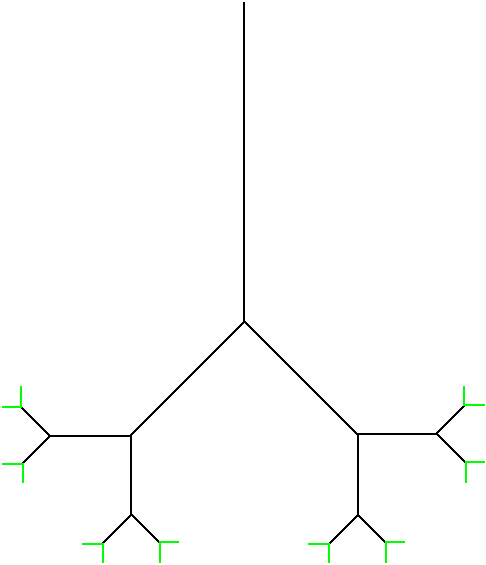
\includegraphics[width=\textwidth]{bintree.png}
Inne przykłady są dostępne w katalogu test\_code, a obrazy wynikowe - w katalogu images.

\section{Formalna specyfikacja}

\subsection{Zdefiniowane tokeny}
\begin{itemize}
    \item{\textit{error} - pomocniczy, w poprawnym kodzie nieużywany}
    \item{\textit{end\_of\_text}}
    \item{\textit{int\_number} - liczba całkowita to: cyfra niezerowa i ciąg cyfr, dozwolony też '-' na początku}
    \item{\textit{float\_number} - na początku liczba całkowtia, potem '.' i ciąg cyfr}
    \item{\textit{literal} - litera, ciąg złożony z liter / cyfr / podkreślników}
    \item{(...)\_\textit{keyword}: forward, rotate, penup, pendown, pencolour, goto, pensize, scale, pushstate, popstate, evaluate, execute, redefine}
    \item{\textit{production\_operator} $->$ }
    \item{\textit{equals\_symbol} = }
    \item{\textit{plus\_symbol} + }
    \item{\textit{l\_curly\_bracket\_symbol} \{ }
    \item{\textit{r\_curly\_bracket\_symbol} \} }
    \item{\textit{l\_round\_bracket\_symbol} ( }
    \item{\textit{r\_round\_bracket\_symbol} ) }
    \item{\textit{semicolon\_symbol} ; }
    \item{\textit{colon\_symbol} , }
\end{itemize}

\subsection{Gramatyka}
Gramatyka opisana po usunięciu komentarzy (jednolinijkowy komentarz zaczynający się od \#). Poniżej - opis gramatyki przed faktoryzacją (bardziej intuicyjny).
\begin{lstlisting}
1: Program = { Statement semicolon_symbol } end_of_text
2: Statement = Definition | Execution
3: Definition = Redefinition | CreateDefinition
4: Execution = LiteralExecution | TurtleStatement
5: LiteralExecution = execute_keyword l_round_bracket_symbol 
                      LiteralString r_round_bracket_symbol
6: Redefinition = redefine_keyword CreateDefinition
7: CreateDefinition = Operation | Production | Evaluation
8: LiteralString = { literal plus_symbol } literal
9: Operation = literal equals_symbol l_curly_bracket_symobl
               { TurtleStatement semicolon_symbol } r_curly_bracket_symbol
10: Production = literal production_operator LiteralString
11: Evaluation = literal equals_symbol evaluate_keyword
                 l_round_bracket_symbol int_number colon_symbol
                 LiteralsString l_round_bracket_symbol
12: TurtleOperation = TurtleOperationKeyword l_round_bracket_symbol
                      TurtleOperationArguments r_round_bracket_symbol
13: TurtleOperationKeyword = forward_keyword | rotate_keyword |
                             penup_keyword | pendown_keyword |
                             pencolour_keyword | goto_keyword |
                             pensize_keyword | scale_keyword |
                             pushstate_keyword | popstate_keyword
14: TurtleOperationArguments = { Number colon_symbol }
15: Number = int_number | float_number
\end{lstlisting}
Różnica w stosunku do dokumentacji wstępnej - zmiana konwencji nazewnictwa i przeniesienie analizy argumentów TurtleOperation na poziom semantyki (parser zaakceptuje dowolny ciąg liczb jako argumenty, a ich poprawność jest sprawdzana poza parserem).
\newline{} \newline{}
Gramatyka po faktoryzacji - łatwa do parsowania (gramatyka regularna):
\begin{lstlisting}
1: Program = { Statement semicolon_symbol } end_of_text
2: Statement = redefine_keyword Redefinition | literal Definition |
               execute_keyword LiteralExecution | 
               TurtleOperationExecution
3: Redefiniton = literal Definition
4: Definition = production_operator Production | 
                equals_symbol OperationOrEvaluation
5: LiteralExecution = l_round_bracket_symbol LiteralString 
                      r_round_bracket_symbol
6: TurtleOperationExecution = TurtleOperation
7: Production = LiteralsString
8: OperationOrEvaluation = l_curly_bracket_symbol Operation |
                           evaluate_keyword Evaluation
9: Operation = { TurtleOperation semicolon_symbol } r_curly_bracket_symbol
10: Evaluaton = l_round_bracket_symbol int_number
                colon_symbol LiteralString l_round_bracket_symbol
11: LiteralString = { literal plus_symbol } literal
12: TurtleOperation = TurtleOperationKeyword l_round_bracket_symbol
                      TurtleOperationArguments r_round_bracket_symbol
13: TurtleOperationKeyword = forward_keyword | rotate_keyword |
                             penup_keyword | pendown_keyword |
                             pencolour_keyword | goto_keyword |
                             pensize_keyword | scale_keyword |
                             pushstate_keyword | popstate_keyword
14: TurtleOperationArguments = { Number colon_symbol }
15: Number = int_number | float_number
\end{lstlisting}

\section{Sposób uruchamiania}
Wymagania: CMake, kompilator C++ (standard co najmniej 11), biblioteka BOOST (do testów jednostkowych), biblioteka SFML (do tworzenia grafiki).
Przykład kompilacji w systemie Linux:
\begin{lstlisting}
rm -rf build
mkdir build
cd build
cmake .. -DCMAKE_BUILD_TYPE=Release
make -j$(nproc)
\end{lstlisting}
Sposób uruchamiania:\newline{}
[ścieżka do programu lturtle] [nazwa pliku wyjściowego]\newline{}
Dane wejściowe (kod do interpretacji) przyjmowane są ze standardowego wejścia. Przykład uruchomienia programu, z przekierowaniem pliku wejściowego:\newline{}
\begin{lstlisting}
./build/lturtle images/bintree.png <test_code/binary_tree  
\end{lstlisting}

\section{Opis sposobu realizacji}

\subsection{Wykorzystane narzędzia}
Program został napisany i przetestowany z wykorzystaniem poniższych narzędzi, ale powinien być przenośny.
\begin{itemize}
    \item{cmake 3.11.1}
    \item{gcc 7.3.1}
    \item{boost 1.66.0-2}
    \item{SFML 2.5.0-1}
    \item{system operacyjny: Manjaro Linux, procesor x86-64}
\end{itemize}

\subsection{Moduły programu}
\begin{itemize}
    \item{exception - zawiera własne klasy wyjątków z "wygodnymi" w użyciu konstruktorami}
    \item{lexer - zawiera pliki source (moduł obsługi źródła), token (struktury danych opisujące pojedynczy token), lexer (analiza leksykalna kodu)}
    \item{parser - zawiera pliki syntax\_tree (opis AST poniżej) i parser (zwraca odpowiednio powiązane ze sobą struktury danych z syntax\_tree)}
    \item{semantics - moduł analizy semantycznej, opisany poniżej}
    \item{main - zawiera funkcję, od której zaczyna się wykonanie główngo programu (jest to oddzielone od reszty programu, aby funkcja main nie była linkowana do testów)}
    \item{tests - testy jednostkowe modułów: lexer, parser, semantics korzystające z biblioteki boost}
\end{itemize}

\subsection{Opis działania}

\textbf{Działanie analizatora leksykalnego}: lekser odczytuje ze źródła kolejne znaki (przy czym po przetworzeniu danego znaku pobiera już kolejny) i zwraca tokeny wymienione w rozdziale 2.1. Token posiada informacje istotne dla semantyki programu (rodzaj tokenu i, w przypadku tokenów literal, int\_number, float\_number - wartość) oraz informację o tym, gdzie się zaczyna i kończy (co jest używane przy podawaniu komunikatu błędu). Uwaga - token int\_number może być traktowany też jako float\_number - wbudowane "rzutowanie". Słowa kluczowe są przechowywane w tablicy haszującej, przy czym wykorzystywana jest "doskonała" funkcja haszująca (brak kolizji i nadmiarowych miejsc w tablicy haszującej - parametry tej funkcji znaleziono w pomocniczym programie hashtest).\newline{}\newline{}
\textbf{Działanie parsera} - ogólna zasada działania jest bardzo podobna do analizatora leksykalnego (ze względu na prostotę języka - gramatyka regularna), z tą różnicą, że z gotowych tokenów budujemy struktury AST. \newline{}

Struktury danych używane w AST:
\begin{itemize}
    \item{Program - ciąg złożony z obiektów dziedziczących po Statement}
    \item{Statement - typ abstrakcyjny}
    \item{Definition : public Statement - typ abstrakcyjny}
    \item{Operation : public Definition - tworzona np. w kodzie: x = { forward(1);}; }
    \item{Production : public Definition - tworzona np. w kodzie: x $->$ x + a;}
    \item{Evaluation : public Definition - tworzona np, w kodzie: a = evaluate(2, x + x);}
    \item{LiteralExecution : public Statement - tworzona np. w kodzie: execute(x);}
    \item{TurtleOperationExecution : public Statement - tworzona np. w kodzie popstate(); (operacja żółwia poza definicją zmiennej)}
    \item{LiteralString, np. x + a}
    \item{TurtleOperation - jedna z operacji zółwia}
    \item{TurtleOperationArguments - argumenty wewnątrz operacji żółwia, np. (255, 0, 0) wewnątrz pencolour()}
\end{itemize}

\textbf{Działanie analizatora semantycznego} - jest podzielone na 2 części.
Pierwsza, następująca równolegle z parsowaniem (jest to możliwe, ponieważ parsowanie kolejnych 'Statement' jest niezależne - unikanie zapisywania AST całego programu to oszczędność pamięci), zapamiętuje kolejne instrukcje żółwia i współrzędne, na których się znalazł, ale niczego nie rysuje. Dzięki temu rozdzielczość obrazu będzie dostosowywana dynamicznie do zakresu współrzędnych, po których przemieszczał się żółw. Rozdzielczość musi być obliczona przed rasteryzacją, ponieważ przyjęcie odgórnie narzuconej rozdzielczości wpływałoby negatywnie na jakość tworzonych obrazów albo znacząco ograniczałoby kreatywność użytkownika w tworzeniu obrazu. W drugiej fazie wykonania (w tym momencie plik z kodem programu może już być zamknięty) następuje rasteryzacja (jedyne, co jest wtedy potrzebne w pamięci, to sam obraz, i ciąg operacji żółwia - każdy program zapisany w LTurtle można sprowadzić do liniowej sekwencji operacji żółwia).\newline{}\newline{}
\textbf{Klasy używane podczas analizy semantycznej}:
\begin{itemize}
    \item{Interpreter - tworzy pozostałe klasy i wywołuje ich główne metody.}
    \item{CodeAnalyzer - klasa używana w pierwszej części analizy semantycznej. Wywołuje parser i interpretuje kolejne 'Statement'. Skutkiem interpretacji Statement może być:}
        \begin{itemize}
            \item{stworzenie lub zmiana definicji (redefine) zmiennej opisanej przez ciąg operacji żółwia ('Operation') lub ewaluację innej zmiennej ('Evaluation') (implementacja tego pierwszego jest trywialna, natomiast stworzenie ewaluacji już nie, ponieważ nie podstawiamy bezpośrednio operacji żółwia z innej zmiennej, tylko zapamiętujemy odnośniki do ewaluowanych zmiennych - dzięki temu po zmianie definicji operacji w danej zmiennej, zmienne wykorzystująe jej ewaluację również będą miały inne operacje)}
            \item{stworzenie lub zmiana definicji podstawienia istniejącej zmiennej ('Production')}
            \item{stworzenie pojedynczej operacji żółwia ('TurtleOperationExecution'), obliczenie jej skutów i zapamiętanie na potrzeby drugiej części interpretacji}
            \item{stworzenie ciągu operacji żółwia podstawionych pod daną zmienną ('LiteralExecution'), obliczenie jej skutów i zapamiętanie na potrzeby drugiej części interpretacji (jeśli zmienna ma operacje żółwia, są one po prostu przepisywane, jeśli natomiast posiada ewalucję, następuje rekurencyjne wywołanie - przerywane, gdy natrafimy już na zwykłe operacje, a nie odnośniki do innych zmiennych)}
        \end{itemize}
    \item{Variable - przechowuje informacje o jednej zmiennej, to znaczy jej produkcję i (operacje żółwia ALBO zmienne opisujące ewaluację). Variable są przechowywane w VariableMap (mapa: string:Variable).}
    \item{TurtleOperation - klasa abstrakcyjna dla różnych rodzajów operacji żółwia, jest to co innego niż TurtleOperation w parserze. TurtleOperation są 'wykonywane' ('apply') w sposób polimorficzny.}
    \item{TurtleState, UtmostTurtleCoordinates, DrawingContext - potrzebne przy wykonywaniu operacji żółwia (TurtleState zarówno w pierwszej jak i drugiej fazie interpetacji, UtmostTurtleCoordinates - tylko w pierwszej, do wyznaczenia skrajnych współrzędnych, DrawingContext - tylko przy rysowaniu).}
\end{itemize}

\textbf{Testowanie}
\begin{itemize}
    \item{tests/lexer\_tests.cpp - testowanie leksera, sprawdzane są wszystkie rodzaje tokenów w różnych konfuguaracjach, a także błędny kod - testy polegają głównie na sprawdzaniu, czy zwrócony został odpowiedni token, z odpowiednią zawartością}
    \item{tests/parser\_tests.cpp - testowanie parsera, sprawdzane są wszystkie rodzaje struktur AST w różnych konfuguaracjach, a także błędny kod - testy polegają głównie na \textbf{wtórnej generacji kodu na podstawie AST} i porównaniu tego z kodem wejściowym (wynik powinien być taki sam, z dokładnością do białych znaków i komentarzy)}
    \item{tests/semantics\_tests.cpp - testowanie analizatora semantycznego, nie są to testy w pełni pokrywające wszystkie możliwe jego użycia - w przypadku ostatniego modułu programu ważniejsze były testy funkcjonalne ("czy program działa")}
    \item{testowanie funkcjonalne - przykładowe kody testujące są dostępne w katalogu test\_code}
\end{itemize}

\section{Możliwe zmiany}

\begin{itemize}
    \item{Napisanie generycznego leksera i parsera (lub skorzystanie z gotowego generatora), co pozwoliłoby np. na swobodne dodawanie nowych słów kluczowych - operacji żółwia.}
    \item{Refaktoryzacja kodu, w szczególności w parserze (sprawdzanie tokenu rozpoczynającego daną strukturę gramatyczną w funkcji parsującej tę strukturę, a nie poza nią).}
    \item{Dokładniejsze testy jednostkowe analizatora semantycznego.}
    \item{Poprawa obsługi błędów - program kończy się po napotkaniu pierwszego błędu i wypisuje, gdzie on wystąpił. W przypadku niektórych błędów składniowych po wystąpieniu błędu można kontynuować parsowanie, a w przypadku niektórych błędów semantycznych - podawać czytelniejsze komunikaty błędów.}
\end{itemize}

\end{document}

